\documentclass[%
 aps, reprint, prl, amsmath,amssymb
]{revtex4-2}

\usepackage{graphicx}% Include figure files
\graphicspath{{figures/}} 
\usepackage{orcidlink}
\usepackage{mathtools}
\usepackage{algpseudocode}

% -------------- arXiv-Style Margin Stamp ----------------
\usepackage[style=iso]{datetime2}
\usepackage{FiraMono} 
\usepackage{tikz}

% Use shipout/background to ensure it stays behind text/figures
\AddToHook{shipout/background}{
  \begin{tikzpicture}[remember picture, overlay]
    \node [
      rotate=90,
      color=gray!80, 
      font=\fontfamily{FiraMono-TLF}\selectfont\footnotesize
    ] at ([xshift=1.2cm]current page.west) {
        WORKING DRAFT \quad $\bullet$ \quad \DTMnow \quad $\bullet$ \quad doi.org/10.17605/OSF.IO/EV8H6 \quad $\bullet$ \quad Homey Music, Corktown, Detroit, USA
    };
  \end{tikzpicture}
}
% --------------------------------------------------------

\DeclareMathOperator*{\argmin}{argmin}

\begin{document}

\title{Information Erasure Inside the Quantum of Action}

\begin{abstract}
Quantum microstates are operationally indistinguishable inside Planck's quantum of action. We show that Landauer's principle compels the erasure of each microstate into the minimal-action state. This erasure granulates the continuum, selecting the discrete configurations of quantum mechanics at low action and smooth classical trajectories at high action.
\end{abstract}


\author{Brian S. Mulloy\orcidlink{0000-0002-1803-3172}}
\email{brian@homeymusic.com}
\affiliation{Computational Complex Systems Laboratory\\Homey Music, Corktown, Detroit, MI, USA}
\date{\today}

\maketitle

\section{De Gosson: The Quantum Blob}

Let a microstate be defined by phase-space coordinates $(q,p)$, where $q$ is position and $p$ is momentum. According to the Heisenberg uncertainty principle \cite{Heisenberg1927}:

\begin{equation}
\label{eq:HeisenbergVariance}
\sigma_q \sigma_p \ge \frac{\hbar}{2}
\end{equation}

\begin{equation}
\label{eq:CovarianceEllipsoid}
\frac{q^2}{2\sigma_q^2} + \frac{p^2}{2\sigma_p^2} \le 1
\end{equation}

\begin{equation}
\label{eq:EllipsoidArea}
A = \pi (\sqrt{2}\sigma_q) (\sqrt{2}\sigma_p) = 2\pi \sigma_q \sigma_p
\end{equation}

Saturating the Heisenberg bound \cite{Heisenberg1927} ($\sigma_q \sigma_p = \hbar/2$) gives the area of the quantum blob $A_b$ \cite{DeGosson2003}:

\begin{equation}
\label{eq:SymplecticCapacity}
A_b = 2\pi \left( \frac{\hbar}{2} \right) = \frac{h}{2}
\end{equation}

\begin{figure}[t!]
    \centering
    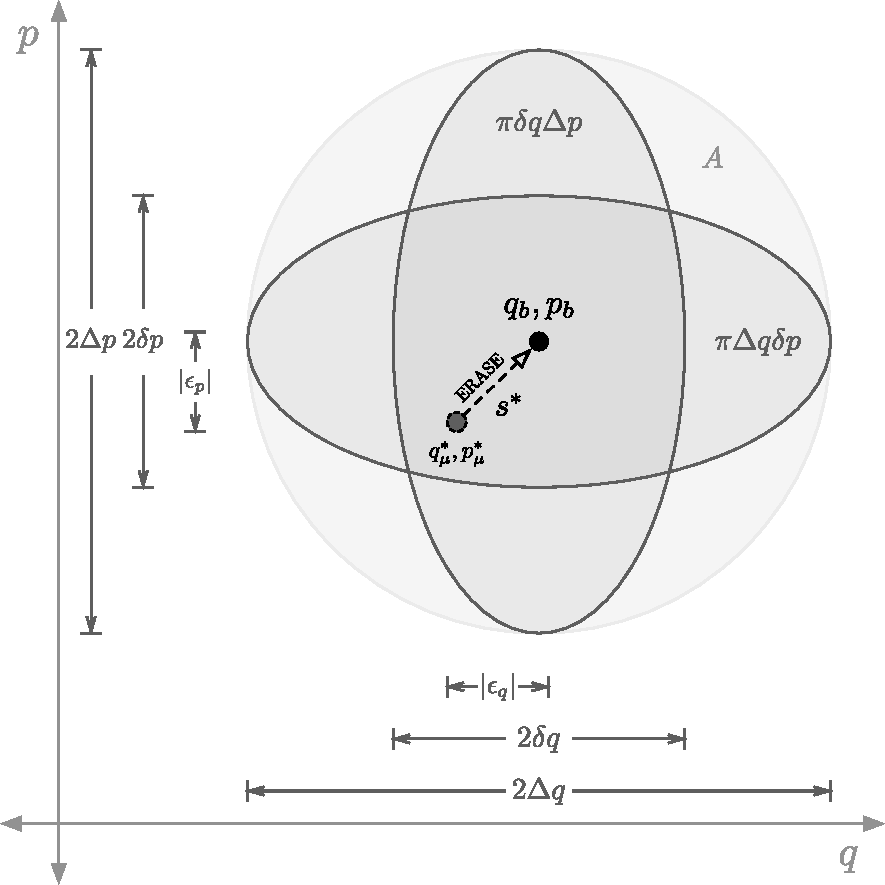
\includegraphics[width=\linewidth]{erase.pdf}
\caption{\textbf{Information erasure inside the quantum of action} (schematic). Boundaries $\Delta q$ and $\Delta p$ determine the classical action area $A$ in phase space. The reciprocal relations $\delta q = \hbar / \Delta p$ and $\delta p = \hbar / \Delta q$ characterize the symplectic squeezing of the conjugate pair of quantum blobs, $\pi \delta q \Delta p = \frac{h}{2}$ and $\pi \Delta q \delta p = \frac{h}{2}$, whose sum is the quantum of action $h$. The values $\epsilon_q$ and $\epsilon_p$ are the erasure distances from each microstate $(q_\mu, p_\mu)$ to the minimal-action state $(q_b,p_b)$ of the blobs. The erasure follows the minimal-action path with binary encoding $s^*$ whose bit count is the Kolmogorov complexity $K = |s^*|$. The physical scales satisfy $|\epsilon_q| \le \delta q \le \Delta q$ and $|\epsilon_p| \le \delta p \le \Delta p$, bounding the erasure action $\frac{A}{h}(\pi |\epsilon_q| \Delta p + \pi \Delta q |\epsilon_p|)$.}
\label{fig:erase_schematic}
\end{figure}

\section{Zurek: One Blob or Two?}

Zurek \cite{Zurek2001} demonstrated that a quantum state constrained by the classical action boundaries $\Delta q$ and $\Delta p$ develops sub-Planck structures defined by the reciprocal limits:

\begin{equation}
\label{eq:BlobSqueeze}
\delta q = \frac{\hbar}{\Delta p} \quad \text{and} \quad \delta p = \frac{\hbar}{\Delta q}
\end{equation}

Expressing Zurek's reciprocal limits as phase-space areas yields a conjugate pair of de Gosson capacities (see Fig.~\ref{fig:erase_schematic}):

\begin{equation}
\label{eq:BlobAreas}
\pi \delta q \Delta p = \frac{h}{2} \quad \text{and} \quad \pi \Delta q \delta p = \frac{h}{2}
\end{equation}

Because both areas are required to bound the space, the total quantum of action $h$ is defined by their sum:

\begin{equation}
\label{eq:SimpleLanguageBlobs}
\text{Quantum of Action} = \text{Pair of Quantum Blobs}
\end{equation}

\begin{equation}
\label{eq:Blobs}
h = \pi \delta q \Delta p + \pi \Delta q \delta p
\end{equation}

\section{Landauer: Information Erasure}

Landauer's principle establishes the minimum thermodynamic cost of information erasure \cite{Landauer1961}:

\begin{equation}
\label{eq:LandauerErasureOneBit}
E_L = k_B T \ln{2}
\end{equation}

The total energy dissipated scales with algorithmic information content, defined as the Kolmogorov complexity $K$ \cite{Kolmogorov1965}:

\begin{equation}
\label{eq:LandauerErasureK}
\text{Total Landauer Cost} = K k_B T \ln{2}
\end{equation}

\section{Margolus-Levitin: Erasure Action}

To express erasure action as a phase-space volume, it is dimensionally necessary to introduce a characteristic erasure time, $\tau$:

\begin{equation}
\label{eq:ErasureActionDefinition}
\text{Erasure Action} = K E_L \tau
\end{equation}

We validate this definition by applying it to the minimal quantum phase space (a de Gosson blob), which is bounded by a minimum action of $h/2$. If this fundamental space is saturated by one position bit and one momentum bit ($K=K_q+K_p=2$), the minimal erasure action is:

\begin{equation}
\label{eq:MinimalErasureAction}
2 E_L \tau = \frac{h}{2}
\end{equation}

Solving for $\tau$ recovers the Margolus-Levitin limit \cite{MargolusLevitin1998} for the minimum time to evolve to an orthogonal state ($\tau_\perp$):

\begin{equation}
\label{eq:MLErasureTime}
\tau_{K=2} = \frac{h}{4 E_L} = \tau_\perp
\end{equation}

This demonstrates that the Margolus-Levitin minimal switching time from above corresponds to the maximal erasure time (e.g., decoherence time) from below.

\section{Lloyd: Erasure Action and Classical Action}

\begin{equation}
\label{eq:ErasureAndClassicalActionPlain}
\text{Erasure Action} \le \text{Classical Action}
\end{equation}

Lloyd demonstrated that the number of elementary logical operations $N$ a physical system can perform in time $t$ is fundamentally bounded by its total available action, $N \le \frac{2 E t}{\pi \hbar}$ \cite{Lloyd2000}. Applying this limit to the geometry of phase space, the total action required to erase $K$ bits of information cannot exceed the classical action capacity, $A$:

\begin{equation}
\label{eq:ErasureAndClassicalAction}
K E_L \tau \le A
\end{equation}

\section{Planck: Quantum Capacity}

Planck demonstrated \cite{Planck1906} that a classical phase space of area $A$ has a capacity of $\Gamma = A/h$ quanta. Scaling the local quantum boundaries ($\delta q, \delta p$) by this macroscopic capacity, we construct the boundaries of the Erasure Action:

\begin{equation}
\label{eq:GeometricActionLimit}
(K_q + K_p) E_L \tau \le \frac{A}{h} (\pi \delta q  \Delta p + \pi \Delta q \delta p)
\end{equation}

Because the minimal-action erasure paths from each microstate to the minimal-action state are bounded by $|\epsilon_q| \le \delta q$ and $|\epsilon_p| \le \delta p$, the erasure action is:

\begin{equation}
\label{eq:ExactGeometricAction}
(K_q + K_p) E_L \tau = \frac{A}{h} (\pi |\epsilon_q| \Delta p + \pi \Delta q |\epsilon_p|)
\end{equation}

\section{Quantum Density from Erasure}

Instead of the Wigner quasi-probability distribution $W(q,p)$ \cite{Wigner1932}, we introduce the Landauer erasure density $L(q,p)$. While Wigner distributions formally possess infinite support, the thermodynamic cost of erasure is dominated by the localized phase-space volume. Therefore, we treat the classical action boundaries $\Delta q$ and $\Delta p$ as operational cutoffs, remaining agnostic to the exponentially vanishing tails of the underlying state:

\begin{equation}
\label{eq:JointErasure}
L(q,p) = \sum_{\mu=1}^{N} \mathbb{I}\left( \frac{A}{h} \epsilon_q = q \right) \mathbb{I}\left( \frac{A}{h} \epsilon_p = p \right)
\end{equation}

\begin{equation}
\label{eq:Marginals}
N(q) = \sum_{p} L(q,p)
\quad \text{and} \quad
N(p) = \sum_{q} L(q,p)
\end{equation}

\begin{figure}[t!]
    \centering
    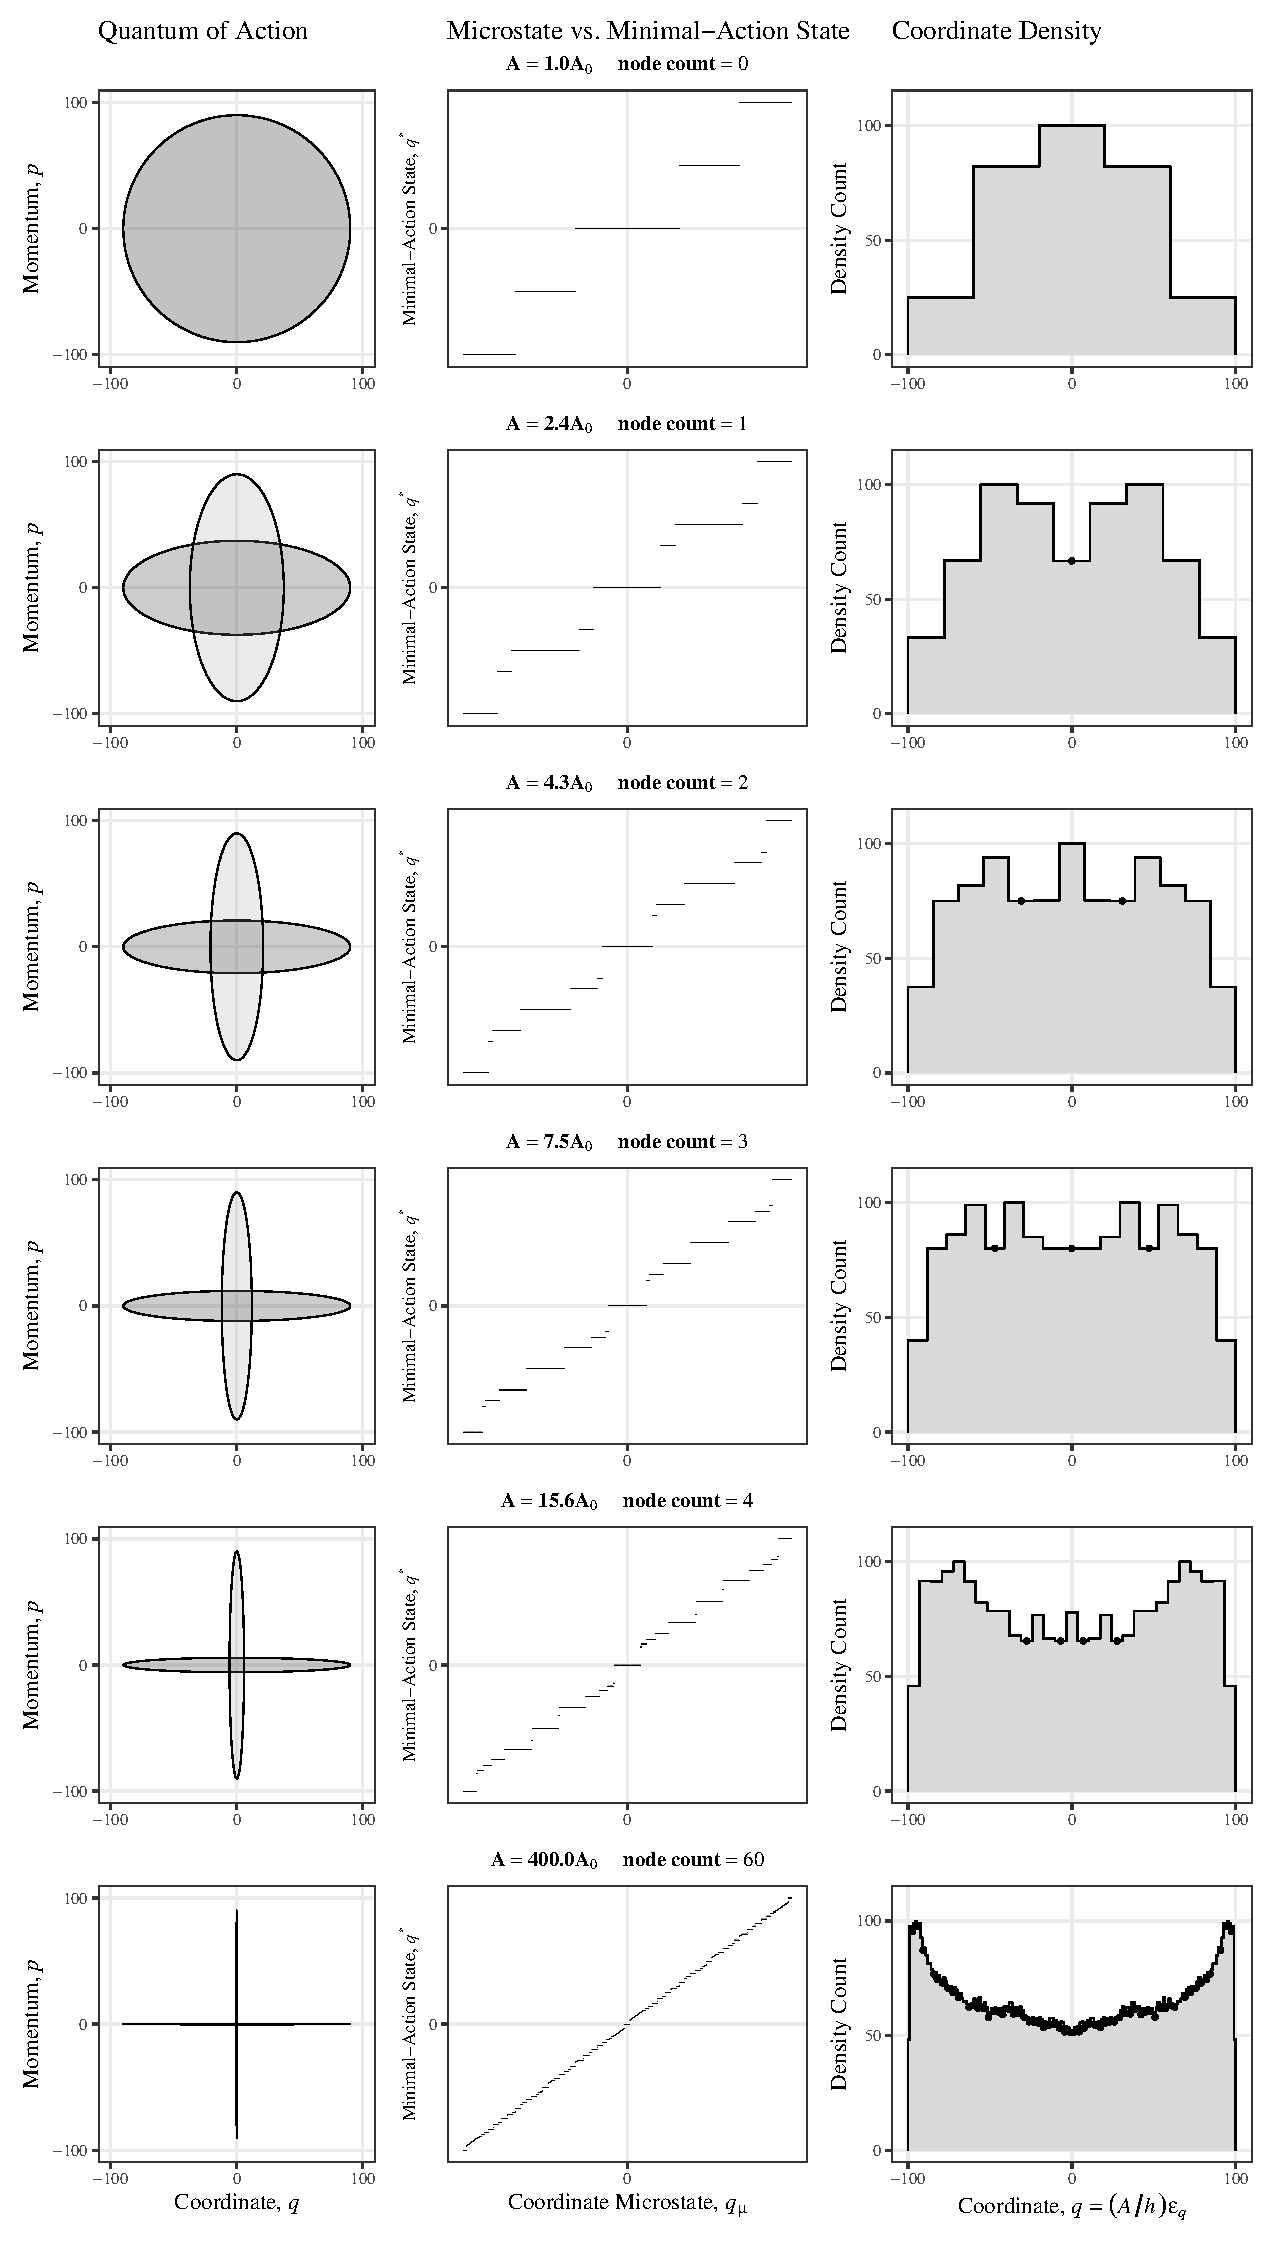
\includegraphics[width=\linewidth]{figures/harmonic_oscillator.pdf}
\caption{\textbf{Harmonic Oscillator Densities from Computation Simulations}.}
\label{fig:harmonic_oscillator}
\end{figure}

\section{Erasure on a Universal Computer}

Let $U$ be a Universal Reversible Turing Machine. A computable encoding function, $\mathcal{E}_U$, encodes the minimal-action microstate $x_\mu$ inside the classical action boundary $\delta x$ centered on the blob component $x_b$ as a binary program string $s_x$:

\begin{equation}
\label{eq:EncoderFunction}
\mathcal{E}_U(x_b, \delta x) \rightarrow (x_\mu, s_x)
\end{equation}

Following Bennett's protocol for logical reversibility \cite{Bennett1973}, we invert and reverse $s_x$ to form the minimal uncomputation path:

\begin{equation}
\label{eq:KolmogorovComplexity}
s_x^* = \operatorname{reverse}(\operatorname{invert}({s_x}))
\end{equation}

Algorithmic erasure of $s_x^*$, where $K_x=|s_x^*|$, incurs Landauer's thermodynamic cost:

\begin{equation}
\label{eq:ErasureFunction}
\texttt{ERASE}(s_x^*) \rightarrow K_x E_L \tau
\end{equation}

Each microstate $(q_\mu, p_\mu)$ uncomputes to $(q_b, p_b)$, creating a displacement in phase space $\epsilon_q = q_\mu - q_b$ and $\epsilon_p = p_\mu - p_b$. The observed macroscopic coordinates $(q,p)$ are those displacements $(\epsilon_q,\epsilon_p)$ scaled by Planck's quantum capacity $A/h$:

\begin{equation}
\label{eq:ObservedCoordinates}
q = \frac{A}{h} \epsilon_q \quad \text{and} \quad p = \frac{A}{h} \epsilon_p
\end{equation}


\section{Numerical Simulations}

We leverage modified sequences \cite{Aiylam2013} to extend the standard Stern-Brocot tree \cite{ConcreteMath} across the entire real line, $\mathbb{R}$, by initializing the search bounds at $\pm \infty$. We simulate the physical encoding function $\mathcal{E}_U$ for any phase-space coordinate, $x \in \{q, p\}$:

\begin{algorithmic}[1]
\Function{$\mathcal{E}_U$}{$x_b, \delta x$}
    \State $\text{left} \gets (-1, 0)$
    \State $\text{num} \gets 0, \quad \text{den} \gets 1$
    \State $x_\mu \gets \text{num} / \text{den}$
    \State $\text{right} \gets (1, 0)$
    \State $s_x \gets \text{``''}$
    \While{$|x_\mu - x_b| > \delta x$}
        \If{$x_\mu < x_b$} 
            \State $\text{left} \gets (\text{num}, \text{den})$
            \State $s_x \gets s_x + \text{``1''}$
        \Else 
            \State $\text{right} \gets (\text{num}, \text{den})$
            \State $s_x \gets s_x + \text{``0''}$
        \EndIf
        \State $\text{num} \gets \text{left}_{\text{num}} + \text{right}_{\text{num}}$
        \State $\text{den} \gets \text{left}_{\text{den}} + \text{right}_{\text{den}}$
        \State $x_\mu \gets \text{num} / \text{den}$
    \EndWhile
    \State \Return $x_\mu, s_x$
\EndFunction
\end{algorithmic}

The minimal program $s_x^*$ is irreversibly destroyed, clearing the tape on $U$:

\begin{algorithmic}[1]
\Function{ERASE}{$s_x^*$}
    \State $K_x \gets |s_x^*|$
    \While{$K_x > 0$}
        \State \Call{ShiftLeft}{$s_x^*$} 
        \Statex \Comment{Dissipate heat $k_B T \ln{2}$ over time $\tau$}
        \State $K_x \gets |s_x^*|$
    \EndWhile
\EndFunction
\end{algorithmic}

\section{A Geometric Uncertainty Principle}

Zurek's Wigner compass demonstrates that quantum interference creates rectangular sub-Planck tiles of area $a = \delta q \delta p$ \cite{Zurek2001}. Generalizing these rectangular bounds to symplectic geometry, we bound this uncertainty within an ellipsoid. 

In the context of phase-space polar duality \cite{deGosson2022}, the unique maximum-volume ellipsoid inscribed within a convex body is the Fritz John ellipsoid \cite{John1948}. While de Gosson's John ellipsoid is saturated at the quantum of action ($h/2$), Zurek's sub-Planck interference forces this inner ellipsoid to be strictly smaller:

\begin{equation}
\label{eq:SubPlanckJohnEllipsoid}
\pi \delta q \delta p \le \frac{h}{2}
\end{equation}

The area of this Fritz John ellipsoid establishes a geometric uncertainty relation bounded by the classical action:

\begin{equation}
\label{eq:GeometricUncertaintyPrinciplePlainLanguage}
\text{Uncertainty} \propto \frac{1}{\text{Classical Action}}
\end{equation}

\begin{equation}
\label{eq:ZurekUncertaintyPrinciple}
\delta q \delta p = \frac{\hbar^2}{\Delta q \Delta p}
\end{equation}

This approach resolves {S}chr{\"{o}}dinger's cat paradox \cite{Schrodinger1980Trimmer}: macroscopic action squeezes quantum uncertainty into fine phase-space crosshairs, enforcing microscopic precision and naturally restoring the correspondence principle.

\section{Ideas to Explore}

\section{Action, Resolution, and Bits}

\begin{equation}
\label{eq:ResolvingPowerPlain}
\substack{\text{Classical} \\ \text{Boundary}}
\propto
\substack{\text{Resolving} \\ \text{Power}} 
\propto
\substack{\text{Bit} \\ \text{Budget}}
\end{equation}

\begin{equation}
\label{eq:BitBudgetResolutionCoordinate}
\Delta p
\propto 
\frac{1}{\delta q} 
\propto 
K_q 
\quad \text{and} \quad
\Delta q
\propto 
\frac{1}{\delta p} 
\propto 
K_p 
\end{equation}

\section{Excess Action}

\begin{equation}
\label{eq:ExcessAction}
\xi_q = \delta q - |\epsilon_q| \quad \text{and} \quad \xi_p = \delta p - |\epsilon_p| 
\end{equation}

\bibliography{main} 
\end{document}